\item \subquestionpointscoding{12} 

Implement both forward-propagation and back-propagation for the above loss function.
Initialize the weights of the network by sampling values from a standard normal
distribution. Initialize the bias/intercept term to 0.
Set the number of hidden units to be 300, and learning rate to be 5. Set $B = 1,000$
(mini batch size). This means that we train with 1,000 examples in each iteration.
Therefore, for each epoch, we need 50 iterations to cover the entire training data.
The images are pre-shuffled. So you don't need to randomly sample the data, and can
just create mini-batches sequentially.


Train the model with mini-batch gradient descent
as described above. Run the training for 30 epochs. At the end of each epoch, calculate
the value of loss function averaged over the entire training set.  To verify a correct implementation, consider plotting the average loss (y-axis) against the number of epochs (x-axis). In the same image, plot the value of the loss function averaged over the dev set, and plot it against the number of epochs.

Similarly, consider plotting the accuracy (on y-axis) over the training set,
measured as the fraction of correctly classified examples, versus the number of epochs
(x-axis). In the same image, plot the accuracy over the dev set versus number of epochs.

Also, at the end of 30 epochs, save the learnt parameters (i.e all the weights and biases)
into a file, so that next time you can directly initialize the parameters with
these values from the file, rather than re-training all over. You do NOT need to
submit these parameters.


\textbf{Hint:} Be sure to vectorize your code as much as possible! Training can be
very slow otherwise.

\clearpage\newpage

You plots should look similar to the following:

\begin{figure}[H]
    \centering
    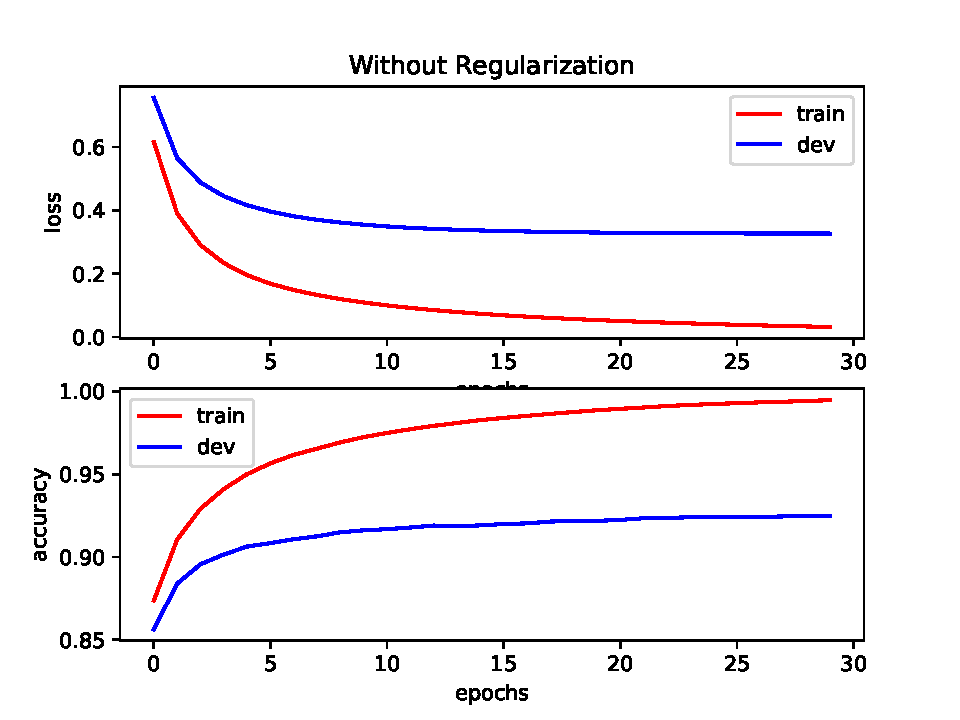
\includegraphics[scale=0.75]{mnist/baseline.pdf}
\end{figure}
